\section{Angles}

\dfnt{Angles particuliers}
{\begin{minipage}{0.45\textwidth}
    On appelle \textbf{angle droit} un angle de 90°. 
    \begin{figure}[H]
        \center
        \begin{tikzpicture}
            \draw (1,0) coordinate (A) -- (-1,0) coordinate (B);
            \draw (0,0) -- (0,1) coordinate (C);
            \draw [gray,right angle quadrant=2,right angle symbol={A}{B}{C}];
        \end{tikzpicture}
    \end{figure}
\end{minipage}
\hfill
\vrule
\hfill
\begin{minipage}{0.45\textwidth}
    On appelle \textbf{angle plat} un angle de 180°.
    \begin{figure}[H]
        \center
        \begin{tikzpicture}
            \draw (3,0) coordinate (a) -- (0,0) coordinate (b) -- (-3,0) coordinate (c);
            \draw pic["180",draw=orange,fill=orange!20,angle eccentricity=1.3, angle radius=0.7cm]{angle=a--b--c};
        \end{tikzpicture}
    \end{figure}
\end{minipage}
}

\prop{Angles opposés}
{\begin{minipage}{0.65\textwidth}
    Soit deux droites. Si :
    \begin{itemize}
        \item Elles sont sécantes 
    \end{itemize}
    Alors les angles formés par leur intersection sont égaux deux à deux avec l'angle opposé.
\end{minipage}
\hfill
\begin{minipage}{0.3\textwidth}
    \begin{figure}[H]
        \center
        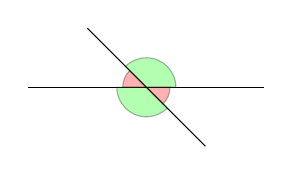
\begin{tikzpicture}[scale=0.75]
            \draw (0,0) -- (4,0) ;
            \draw (1,1) -- (3,-1) ;
            \draw [fill=green, opacity=0.3] (2.5,0) arc (0:135:0.5)--(2,0)--cycle;
            \draw [fill=green, opacity=0.3] (1.5,0) arc (180:315:0.5)--(2,0)--cycle;
            \draw [fill=red, opacity=0.3] (2.4,0) arc (0:-45:0.4)--(2,0)--cycle;
            \draw [fill=red, opacity=0.3] (1.6,0) arc (180:135:0.4)--(2,0)--cycle;
        \end{tikzpicture}
    \end{figure}
\end{minipage}
}

\prop{Somme des angles d'un triangle}
{La somme des trois angles d'un triangle est égale à 180°.}

\prop{Angles alternes-internes}
{\begin{minipage}{0.68\textwidth}
    Soient trois droites $(a),(b)$ et $(c)$. Si :
\begin{itemize}
    \item $(a)$ et $(b)$ sont parallèles.
    \item $(c)$ coupe les droites $(a)$ et $(b)$
\end{itemize}
Alors les angles alternes internes formés par l'intersection de $(a)$ et $(c)$ et ceux de l'intersection de $(b)$ et $(c)$ sont de même mesure.
\end{minipage}
\hfill
\begin{minipage}{0.3\textwidth}
    \begin{figure}[H]
        \center
        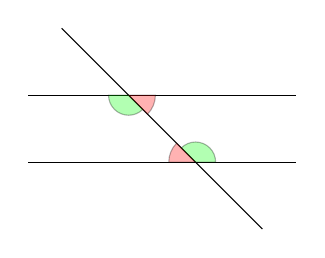
\begin{tikzpicture}[scale=0.85]
            \draw (-0.5,0) -- (3.5,0) ;
            \draw (0,2) -- (3,-1) ;
            \draw (-0.5,1) -- (3.5,1) ;
            \draw [fill=green, opacity=0.3] (2.3,0) arc (0:135:0.3)--(2,0)--cycle;
            \draw [fill=green, opacity=0.3] (0.7,1) arc (180:315:0.3)--(1,1)--cycle;
            \draw [fill=red, opacity=0.3] (1.6,0) arc (180:135:0.4)--(2,0)--cycle;
            \draw [fill=red, opacity=0.3] (1.4,1) arc (0:-45:0.4)--(1,1)--cycle;
        \end{tikzpicture}
    \end{figure}
\end{minipage}
}

\prop{Angles alternes-internes-réciproque}
{\begin{minipage}{0.65\textwidth}
    Soient trois droites $(a),(b)$ et $(c)$. Si :
    \begin{itemize}
        \item $(c)$ coupe les droites $(a)$ et $(b)$
        \item Les angles alternes internes sont de même mesure
    \end{itemize}
    Alors les droites $(a)$ et $(b)$ sont parallèles.
\end{minipage}
\hfill
\begin{minipage}{0.3\textwidth}
    \begin{figure}[H]
        \center
        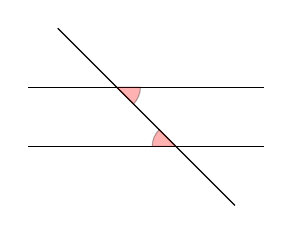
\begin{tikzpicture}[scale=0.75]
            \draw (-0.5,0) -- (3.5,0) ;
            \draw (0,2) -- (3,-1) ;
            \draw (-0.5,1) -- (3.5,1) ;
            \draw [fill=red, opacity=0.3] (1.6,0) arc (180:135:0.4)--(2,0)--cycle;
            \draw [fill=red, opacity=0.3] (1.4,1) arc (0:-45:0.4)--(1,1)--cycle;
        \end{tikzpicture}
    \end{figure}
\end{minipage}
}

\rmq{Une égalité suffit.}